\subsection{Relative Jet Energy Scale}

\subsubsection{Measurement} 

The dijet \pt-balance technique, described in Section~\ref{sec:methods}, is used to measure the response of a jet at any $\eta$ relative to the jet energy response in the region $|\eta|<1.3$. Figure~\ref{fig:balance} shows example distributions of the balance quantity $\mathcal{B}$ for PF jets in two pseudorapidity bins. Figure~\ref{fig:relrsp} shows the relative response as a function of $\eta$ in the range $100\GeV < \ptave < 130\GeV$. Ideally, the relative response of the corrected jets in the simulation should be equal to unity. However, because of the resolution bias effect (Section~\ref{sec:resbias}), the relative response in the simulation is found to deviate from unity by an amount equal to the resolution bias. The comparison of the data with the MC simulations implicitly assumes that the resolution bias in the data is the same as in the simulation. This assumption is the dominant systematic uncertainty related to the measurement of the relative response with the dijet balance method.

\begin{figure}[ht!]
  \begin{center}
    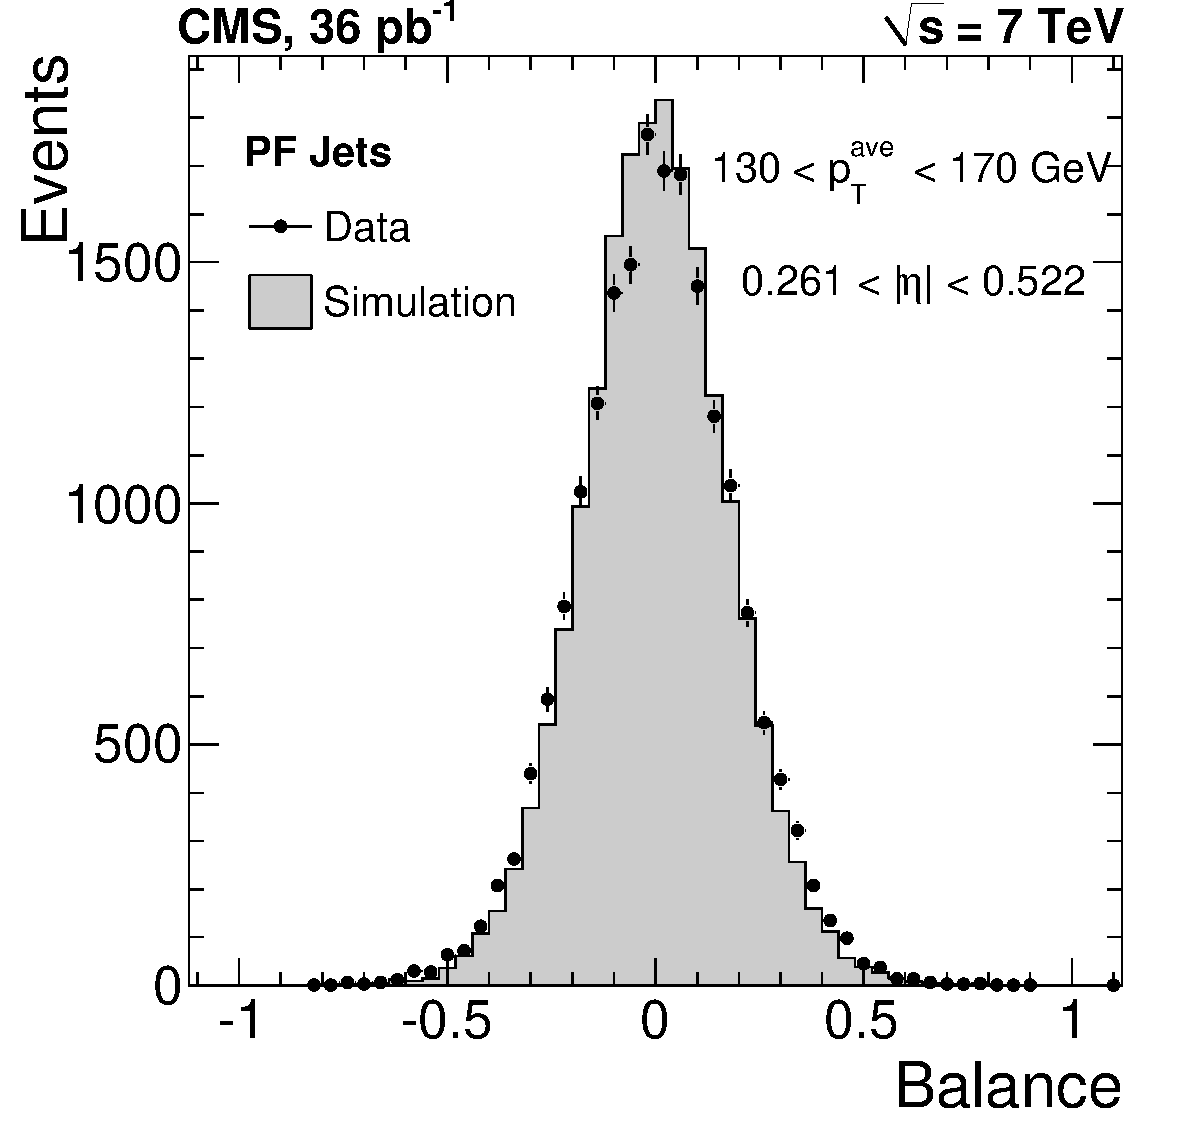
\includegraphics[width=0.45\textwidth]{Figures/JEC/B_DijetPt4_Eta1_ak5pfl1l2l3}
    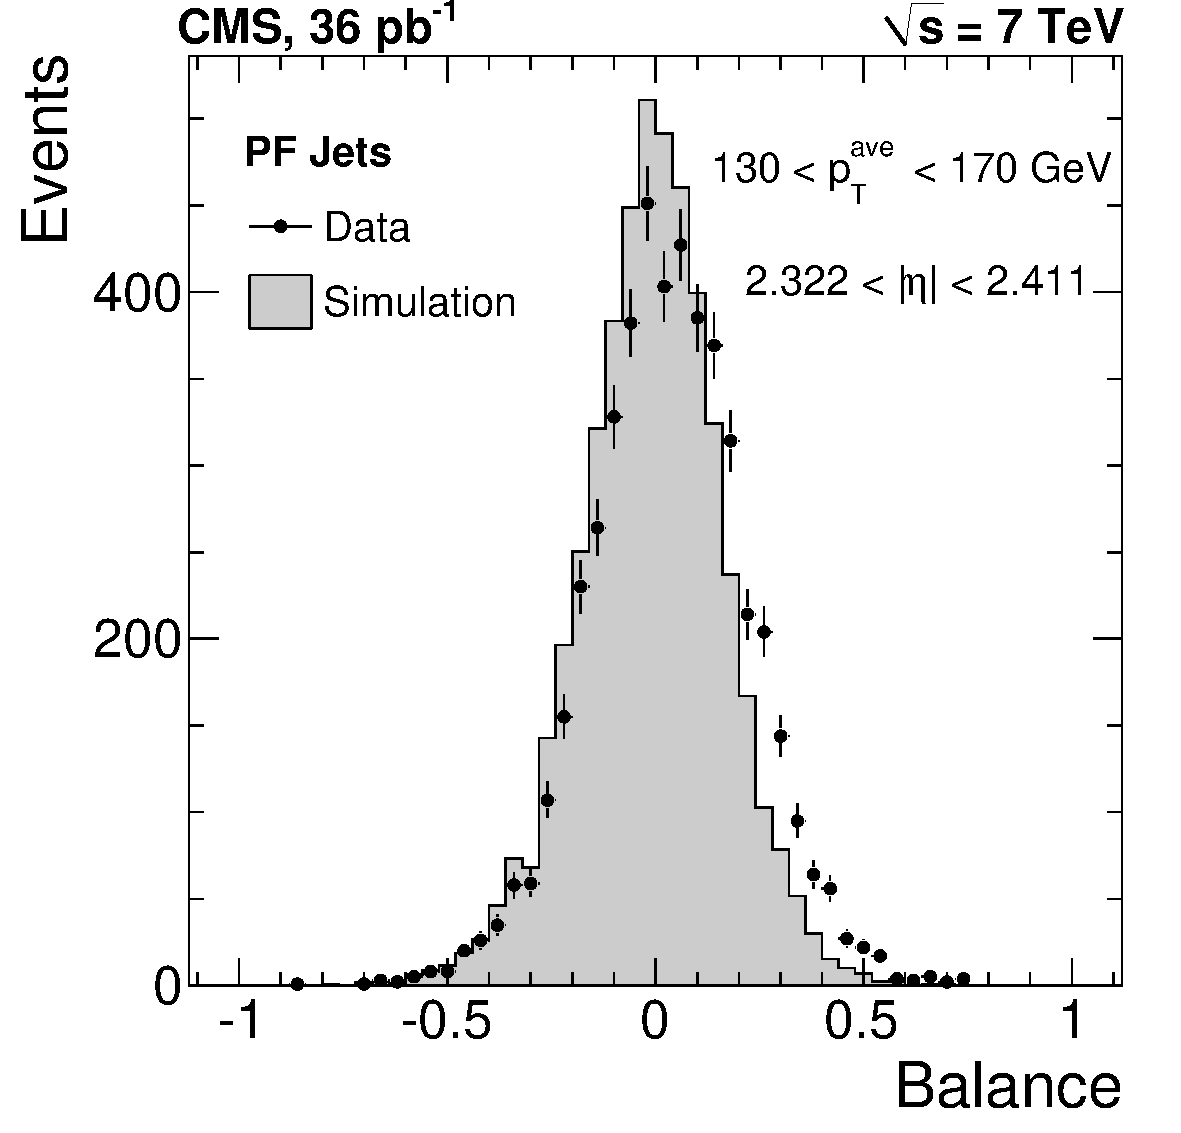
\includegraphics[width=0.45\textwidth]{Figures/JEC/B_DijetPt4_Eta9_ak5pfl1l2l3}
    \caption{Example distributions of the dijet balance quantity for PF jets in two $\eta$ regions.}
    \label{fig:balance}
  \end{center}
\end{figure}

\begin{figure}[ht!]
  \begin{center}
    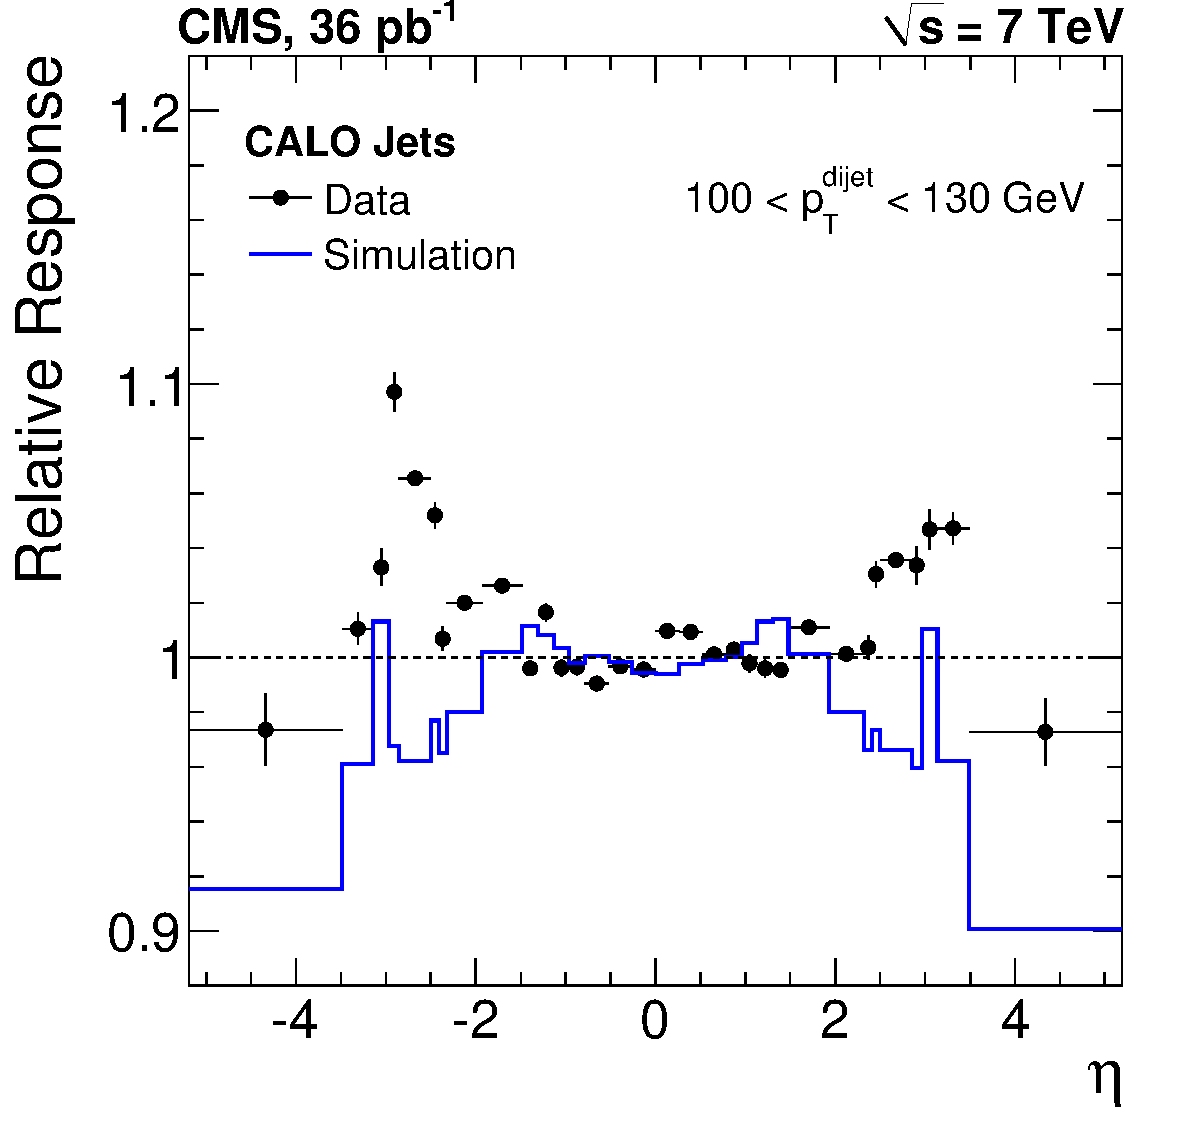
\includegraphics[width=0.45\textwidth]{Figures/JEC/RelativeResponse_Pt3_ak5calol1l2l3}
    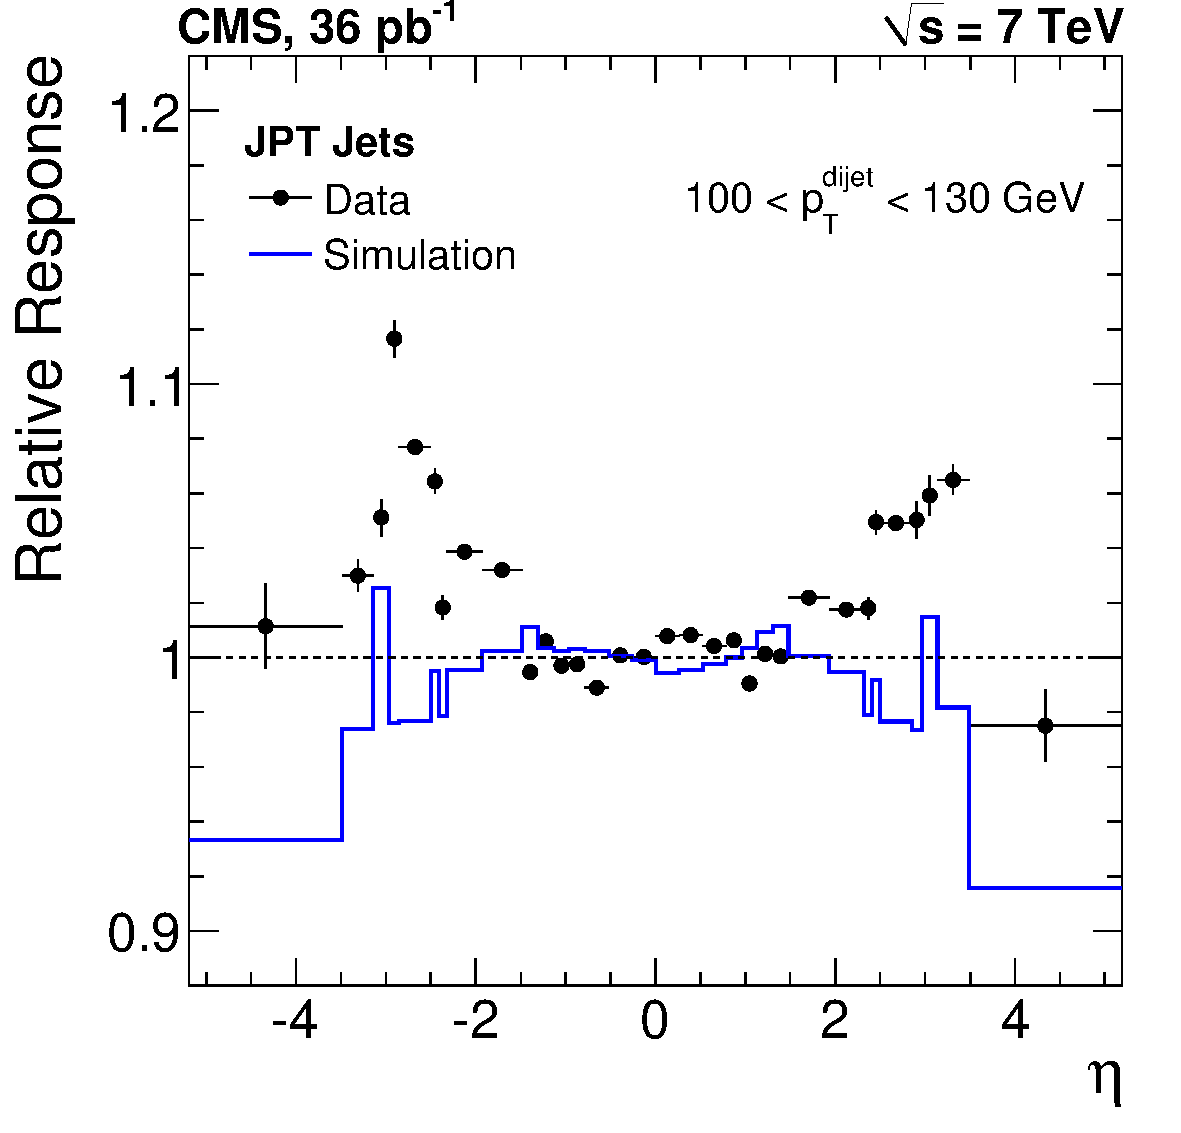
\includegraphics[width=0.45\textwidth]{Figures/JEC/RelativeResponse_Pt3_ak5jptl1l2l3}
    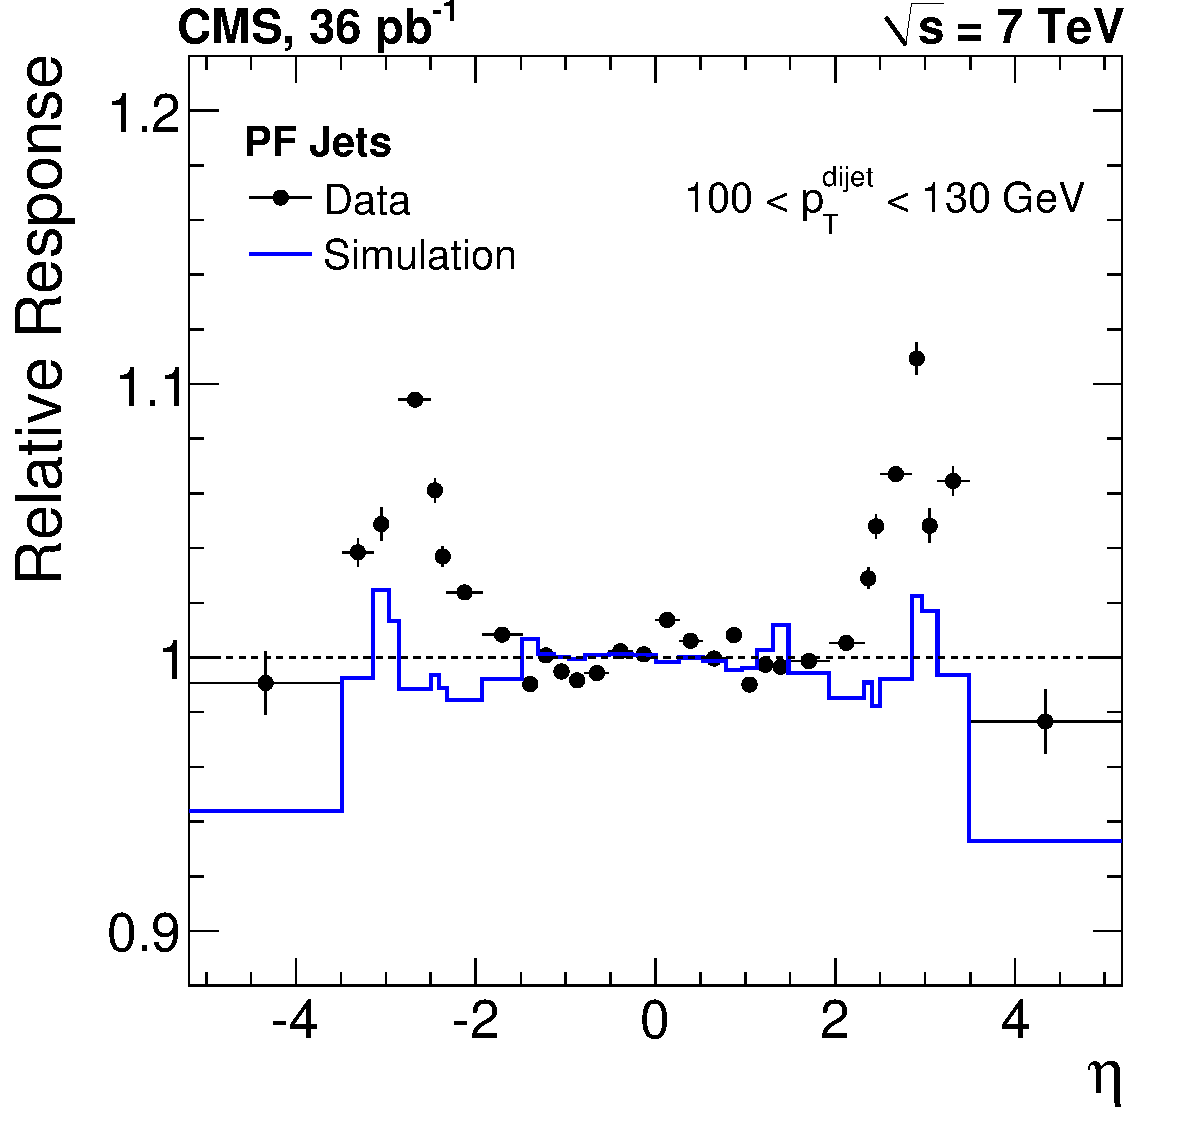
\includegraphics[width=0.45\textwidth]{Figures/JEC/RelativeResponse_Pt3_ak5pfl1l2l3}
    \caption{Relative jet energy response as a function of $\eta$, measured with the dijet balance method for CALO, JPT and PF jets respectively.}
    \label{fig:relrsp}
  \end{center}
\end{figure}

In order to reduce the radiation bias (Section~\ref{sec:radbias}), a selection is applied on the ratio $\alpha=\ptthird/\ptave$ and the nominal analysis value is $\alpha<0.2$. The residual relative correction calculation is done in three steps: first, the $\eta$-symmetric part, $C_\text{sym}$, is measured in bins of $|\eta|$, in order to maximize the available statistics, with the nominal requirement $\alpha<0.2$. Then, a correction factor $k_\text{rad}$ is applied to take care of the extrapolation to $\alpha=0$, and finally the asymmetry in $\eta$, $\mathcal{A}_R(|\eta|)$, is taken into account. The residual correction for the relative jet energy scale is formally expressed below:

\begin{equation}
  C_\text{rel}(\pm\eta) = \frac{k_\text{rad}(|\eta|)\cdot C_\text{sym}(|\eta|)}{1\mp \mathcal{A}_R(|\eta|)}.
\end{equation}

The $C_\text{sym}$ component is defined by comparing the relative response in data and MC simulations: 

\begin{equation}
  C_\text{sym}(|\eta|) = \left<\frac{R_{MC}^{\alpha<0.2}}{R_{data}^{\alpha<0.2}}\right>_{\pt},
\end{equation}

averaged over the entire \pt range. This is justified by the fact that no statistically significant \pt-dependence is observed in the comparison between data and simulation.

Since the additional radiation and the UE are not perfectly modeled in the simulation, a correction needs to be applied by extrapolating to zero third-jet activity, as discussed in Section~\ref{sec:radbias}. The radiation correction $k_{rad}$ is defined as: 

\begin{equation}
  k_\text{rad} = \lim_{\alpha\to 0}\left(\dfrac{\left<\frac{R_{MC}^\alpha}{R_{data}^\alpha}\right>_{\pt}}{\left<\frac{R_{MC}^{\alpha<0.2}}{R_{data}^{\alpha<0.2}}\right>_{\pt}}\right).
\end{equation}

Figure~\ref{fig:FSR} (left) shows the radiation correction that needs to be applied to the measurement at the working point $\alpha<0.2$. The correction is negligible in the central region while it reaches the value of 3\% at larger rapidities.

\begin{figure}[ht!]
  \begin{center}
    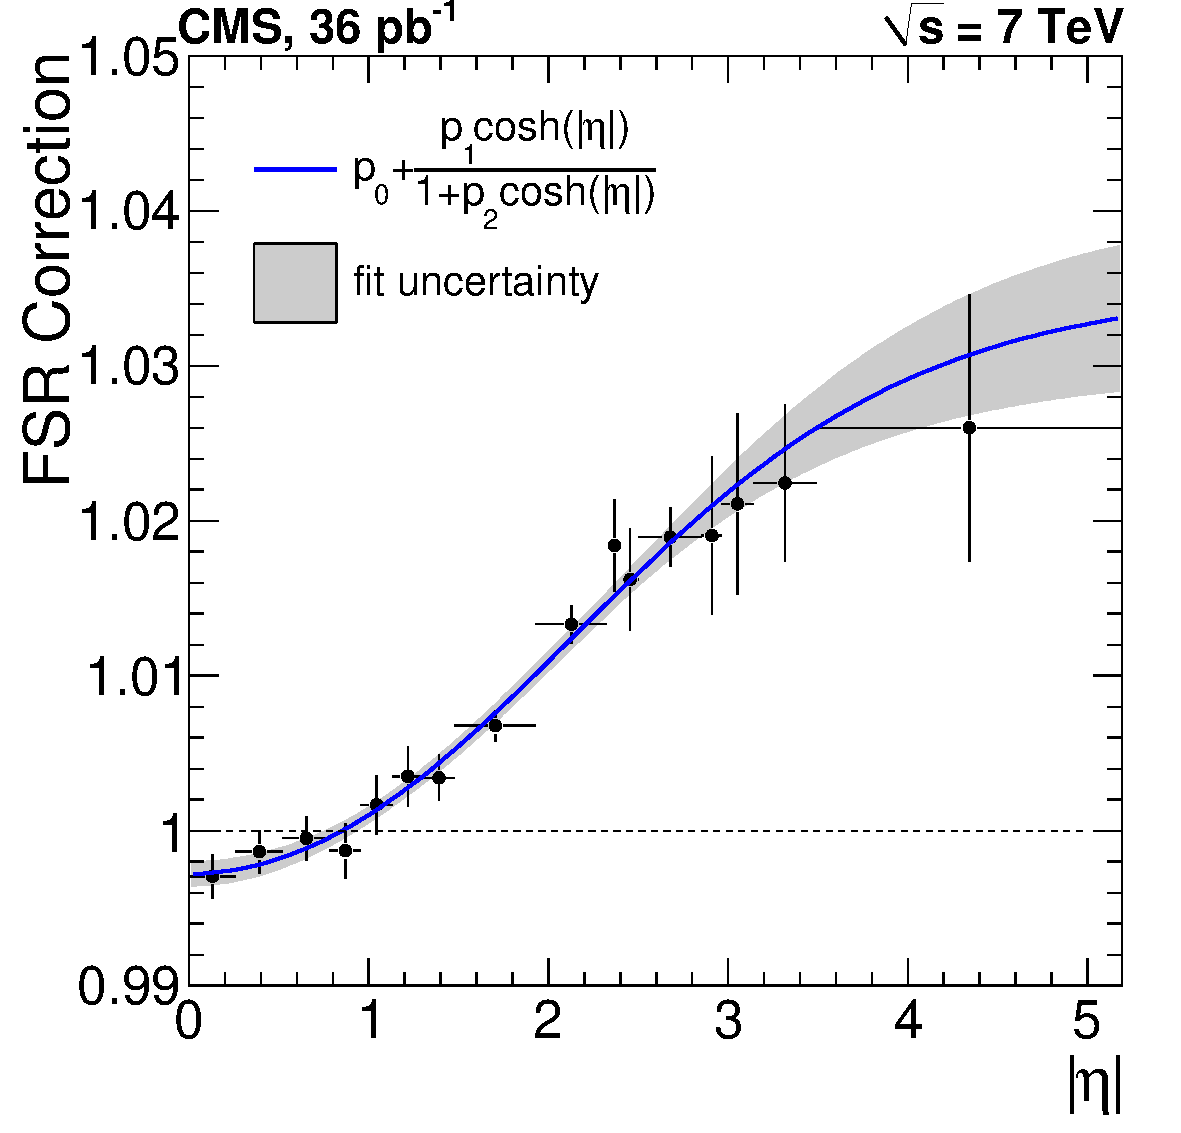
\includegraphics[width=0.45\textwidth]{Figures/JEC/FSR}
    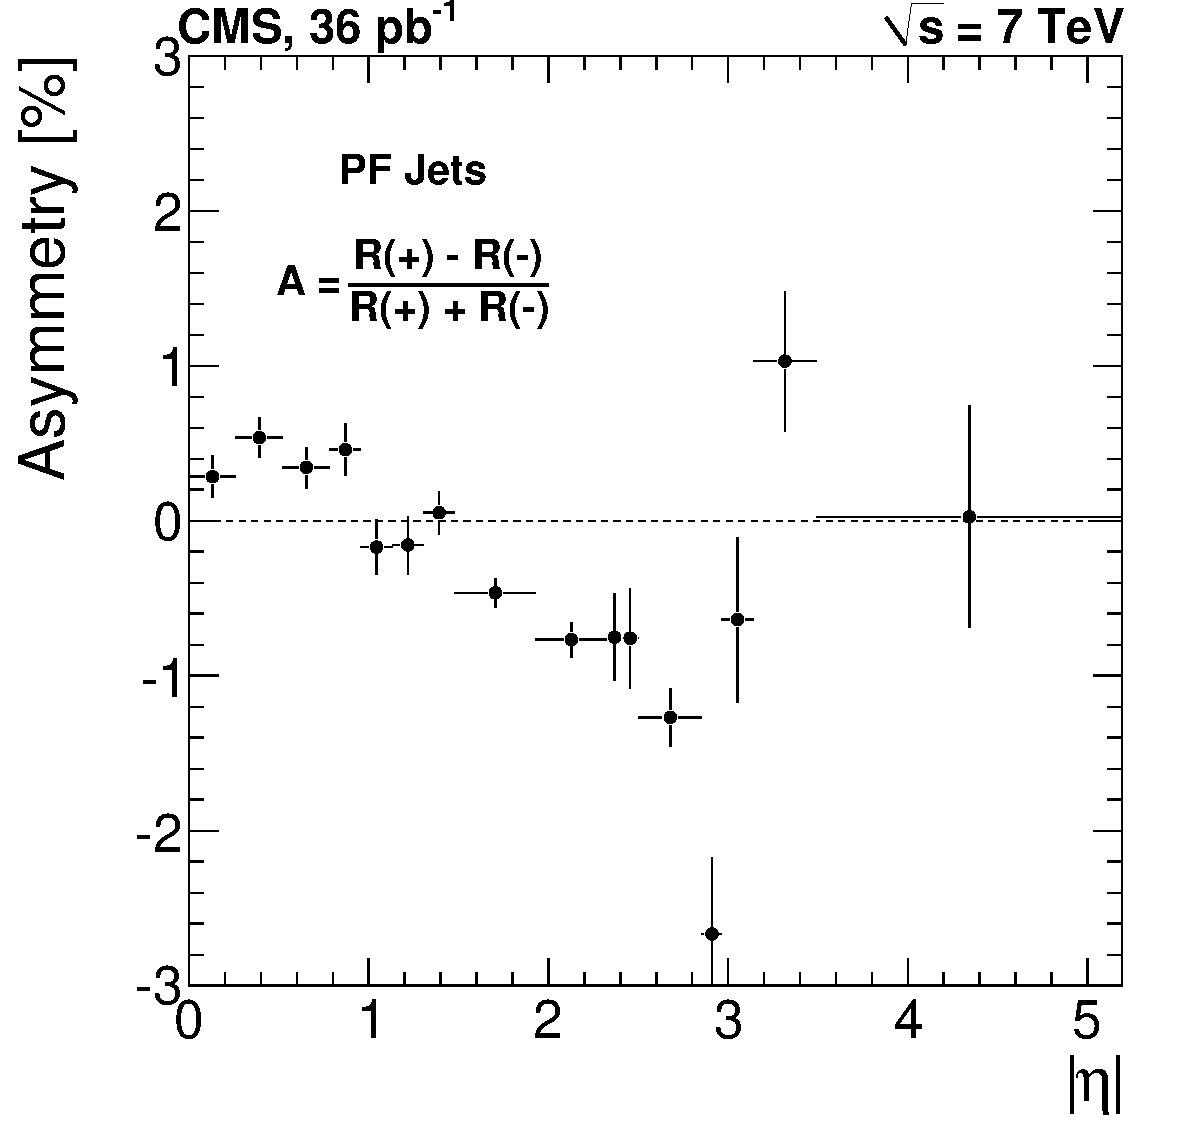
\includegraphics[width=0.45\textwidth]{Figures/JEC/AsymmetryVsEta_ak5pfl1l2l3}
    \caption{Left: correction $k_\text{rad}$ of the relative jet energy residual due to initial and final state radiation. Right: relative jet energy response asymmetry as a function of jet $|\eta|$, for $\alpha<0.2$.}
    \label{fig:FSR}
  \end{center}
\end{figure}

The asymmetry of the response in $\eta$ is quantified through the variable $\mathcal{A}_R$:

\begin{equation}
  \mathcal{A}_R(|\eta|) = \frac{R(+|\eta|)-R(-|\eta|)}{R(+|\eta|)+R(-|\eta|)},
\end{equation}

where $R(+|\eta|)$ ($R(-|\eta|)$) is the relative response measured in the data at the detector part lying in the direction of the positive (negative) z-axis. Figure~\ref{fig:FSR} (right) shows the measured asymmetry. It is found to be similar for the different jet types.

Figure~\ref{fig:final_residual} shows the final residual correction, as a function of $\eta$, for all jet types. This correction is typically of the order of 2-3\%, with the exception of the region $2.5<|\eta|<3.0$ where it reaches the value of 10\%. The region where the larger discrepancy between data and MC simulations is observed (Fig.~\ref{fig:relrsp}), coincides with the border between the endcap and the forward calorimeters. It has also been observed~\cite{JME-10-008} that the single-particle response shows similar behavior in this region.

\begin{figure}[ht!]
  \begin{center}
    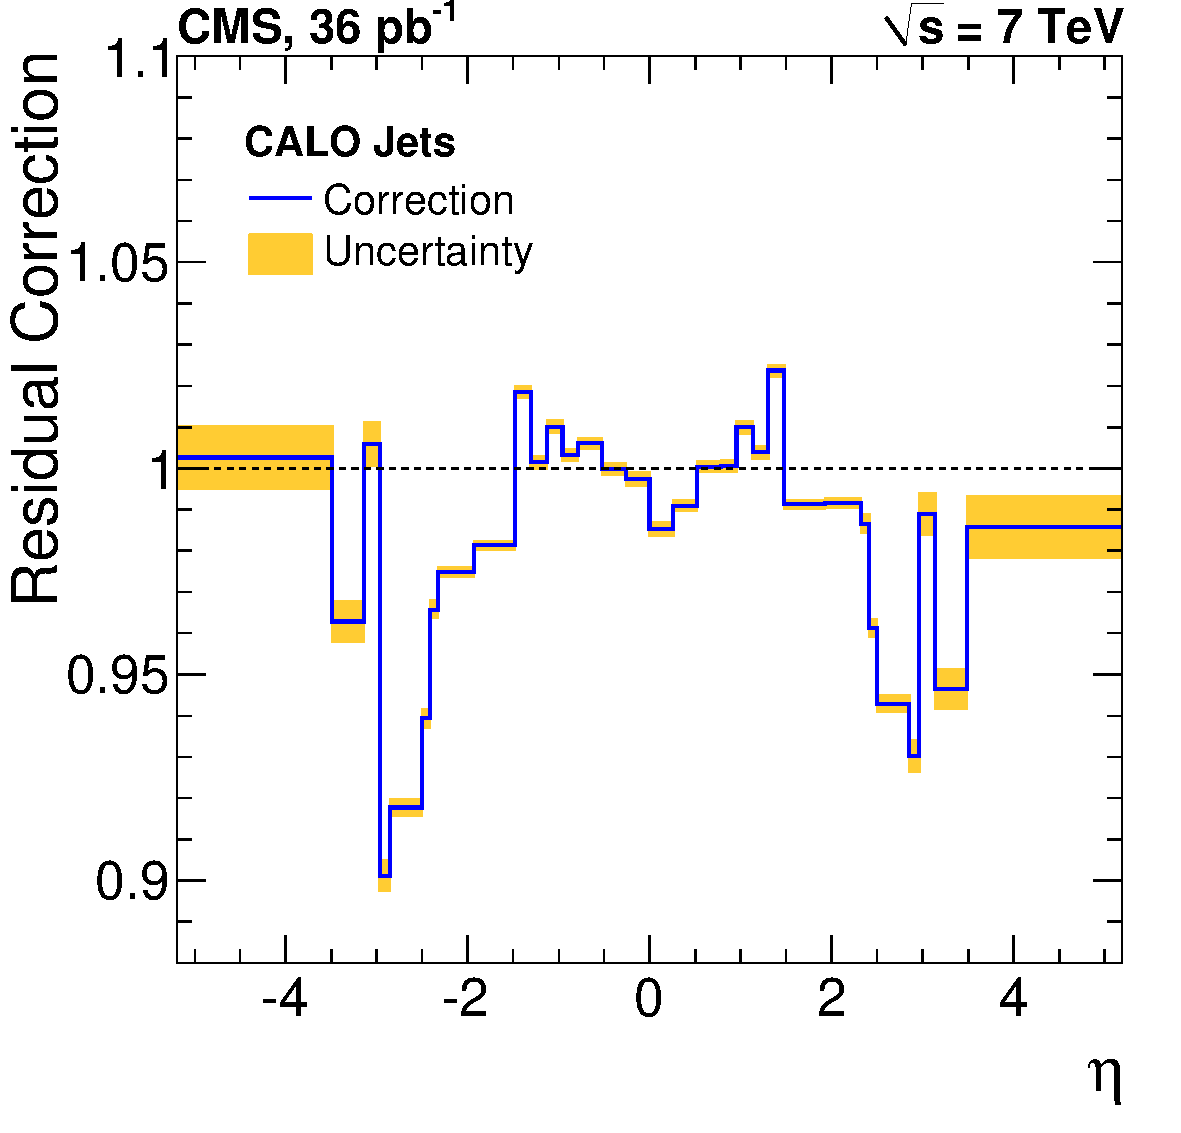
\includegraphics[width=0.45\textwidth]{Figures/JEC/FinalResidual_ak5calol1l2l3}
    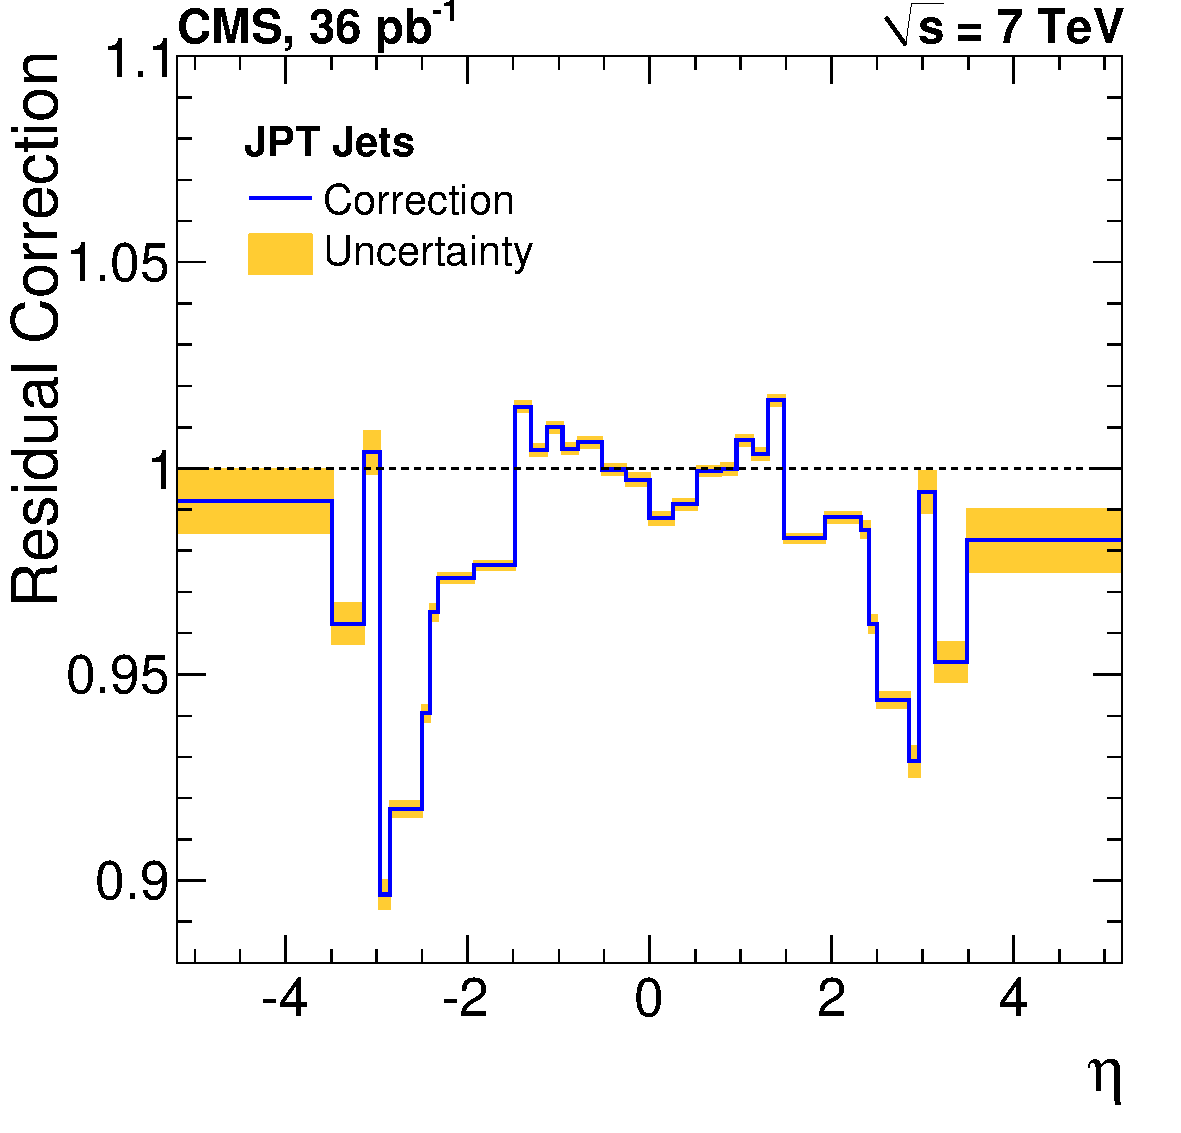
\includegraphics[width=0.45\textwidth]{Figures/JEC/FinalResidual_ak5jptl1l2l3}
    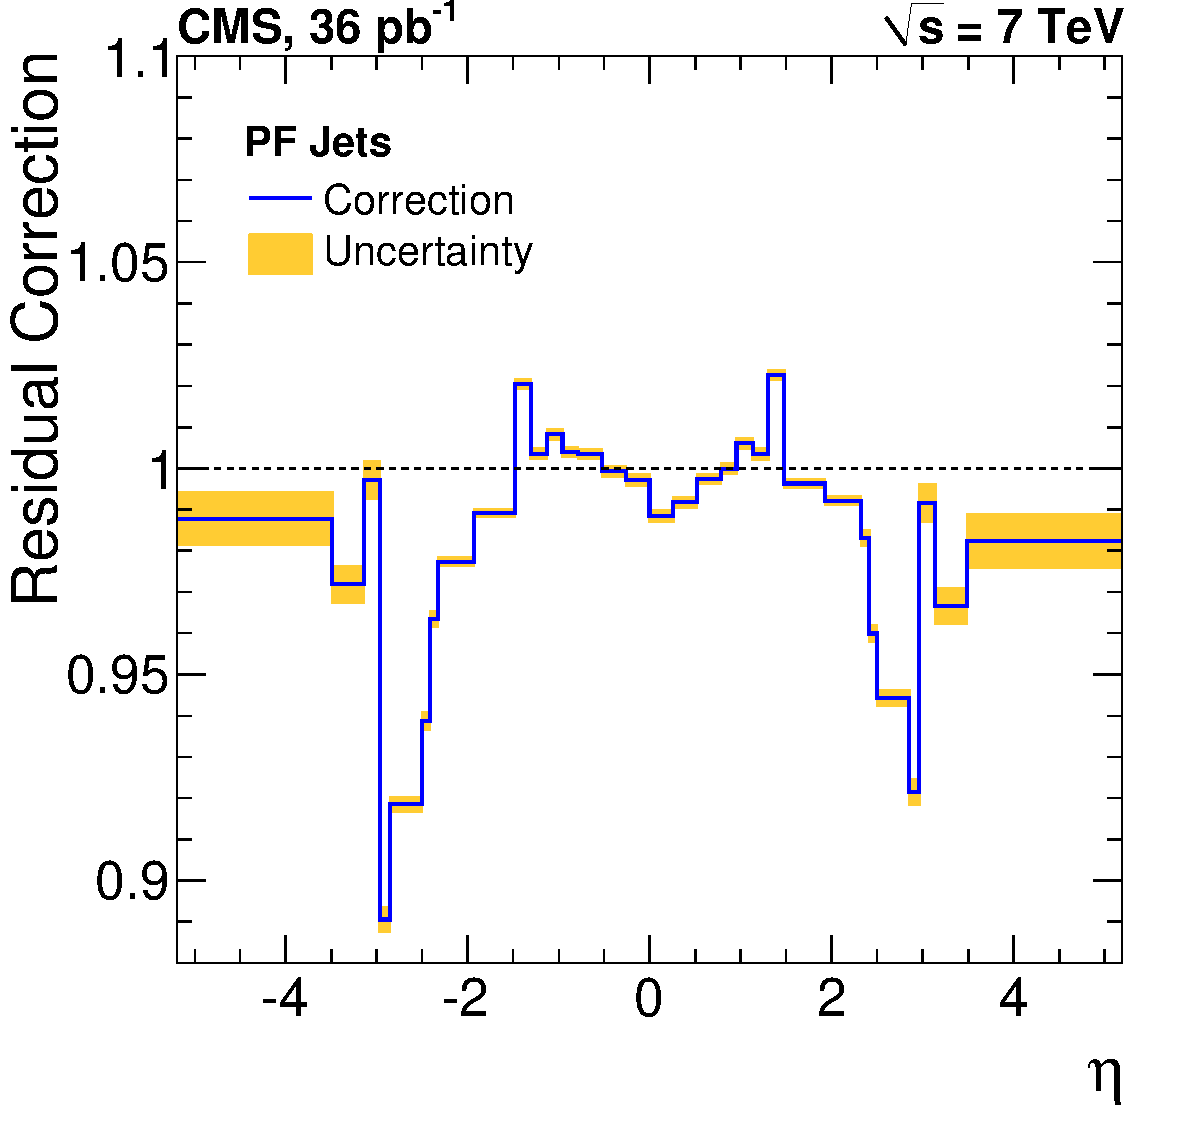
\includegraphics[width=0.45\textwidth]{Figures/JEC/FinalResidual_ak5pfl1l2l3}
    \caption{Relative jet energy residual correction as a function of jet $\eta$ for CALO, JPT and PF jets respectively. The band shows the uncertainty due to statistics, radiation corrections, and asymmetry in $\eta$.}
    \label{fig:final_residual}
  \end{center}
\end{figure}

Finally, Fig.~\ref{fig:L2Closure} demonstrates that the derived residual correction establishes an almost perfect agreement between data and simulation.

\begin{figure}[ht!]
  \begin{center}
    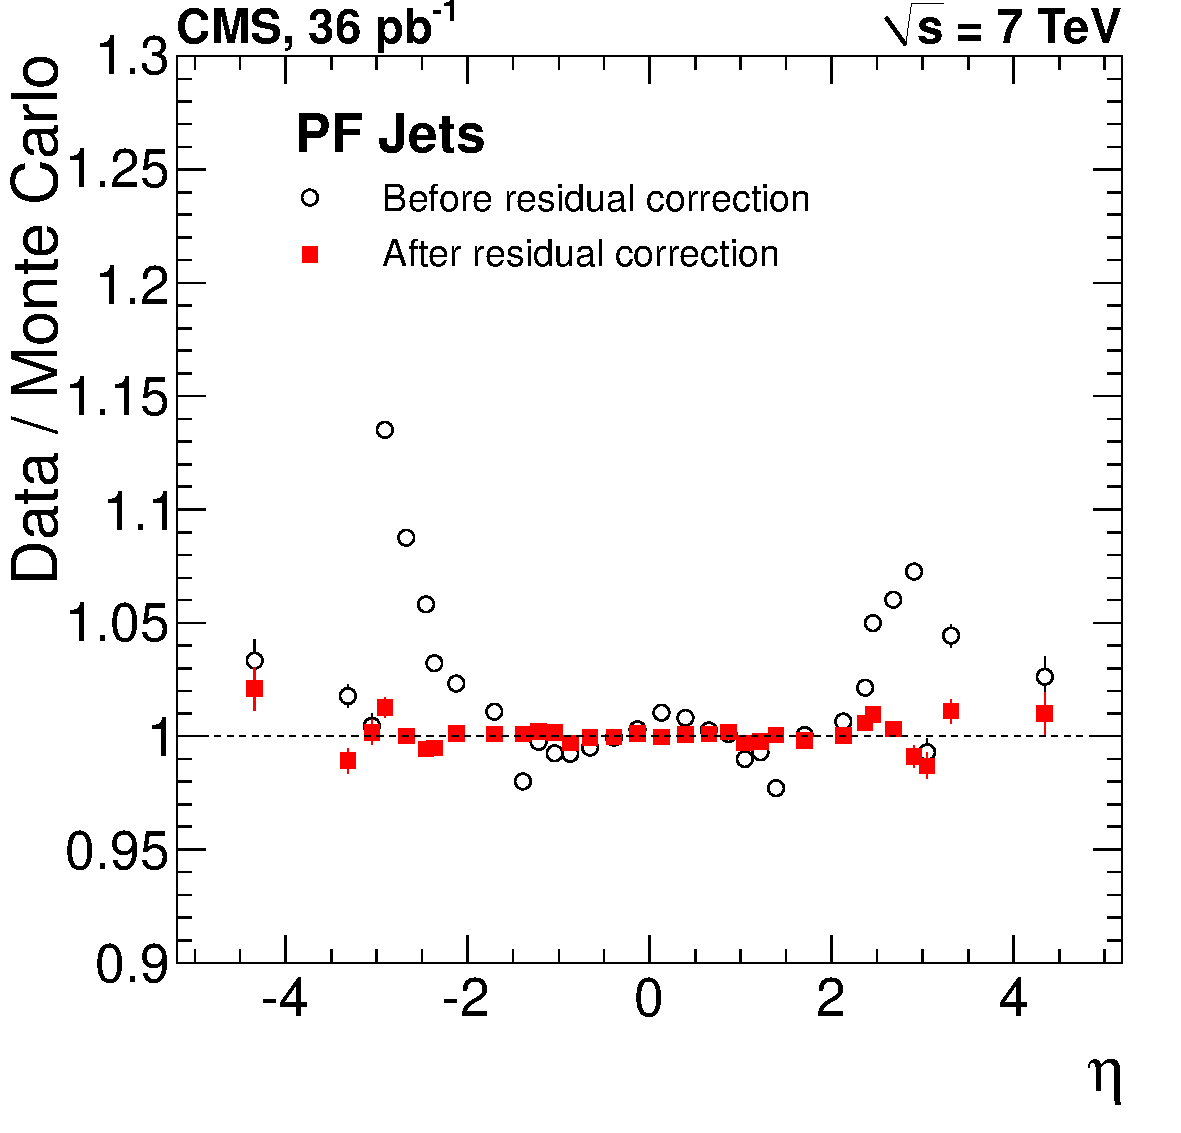
\includegraphics[width=0.45\textwidth]{Figures/JEC/RelResponseClosurePF.pdf}
    \caption{Relative response ratio between data and MC simulation before and after the residual correction.}
    \label{fig:L2Closure}
  \end{center}
\end{figure}

\subsubsection{Uncertainty}

The dominant uncertainty of the relative residual correction is due to the simulation of the jet energy resolution, which defines the magnitude of the resolution bias. The estimate of the systematic uncertainty is achieved by varying the jet \pt resolution according to the comparisons between data and MC simulations shown in Section~\ref{sec:res}. Other sources of uncertainty, such as lack of available events, radiation correction and asymmetry in $\eta$ are found to be smaller than 1\%. The total uncertainty of the relative jet energy scale is shown in Fig.~\ref{fig:residual_unc} as a function of the jet $|\eta|$ for two characteristic values of jet \pt (50\GeV, 200\GeV). The CALO jets have systematically larger uncertainty, as opposed to PF jets which have the smallest while the JPT jets uncertainty lies between the values for the other two jet types. This pattern is consistent with the behavior of the jet energy resolution. Also, it is observed that the relative scale uncertainty grows toward larger rapidities because of the larger resolution uncertainty. 

\begin{figure}[ht!]
  \begin{center}
    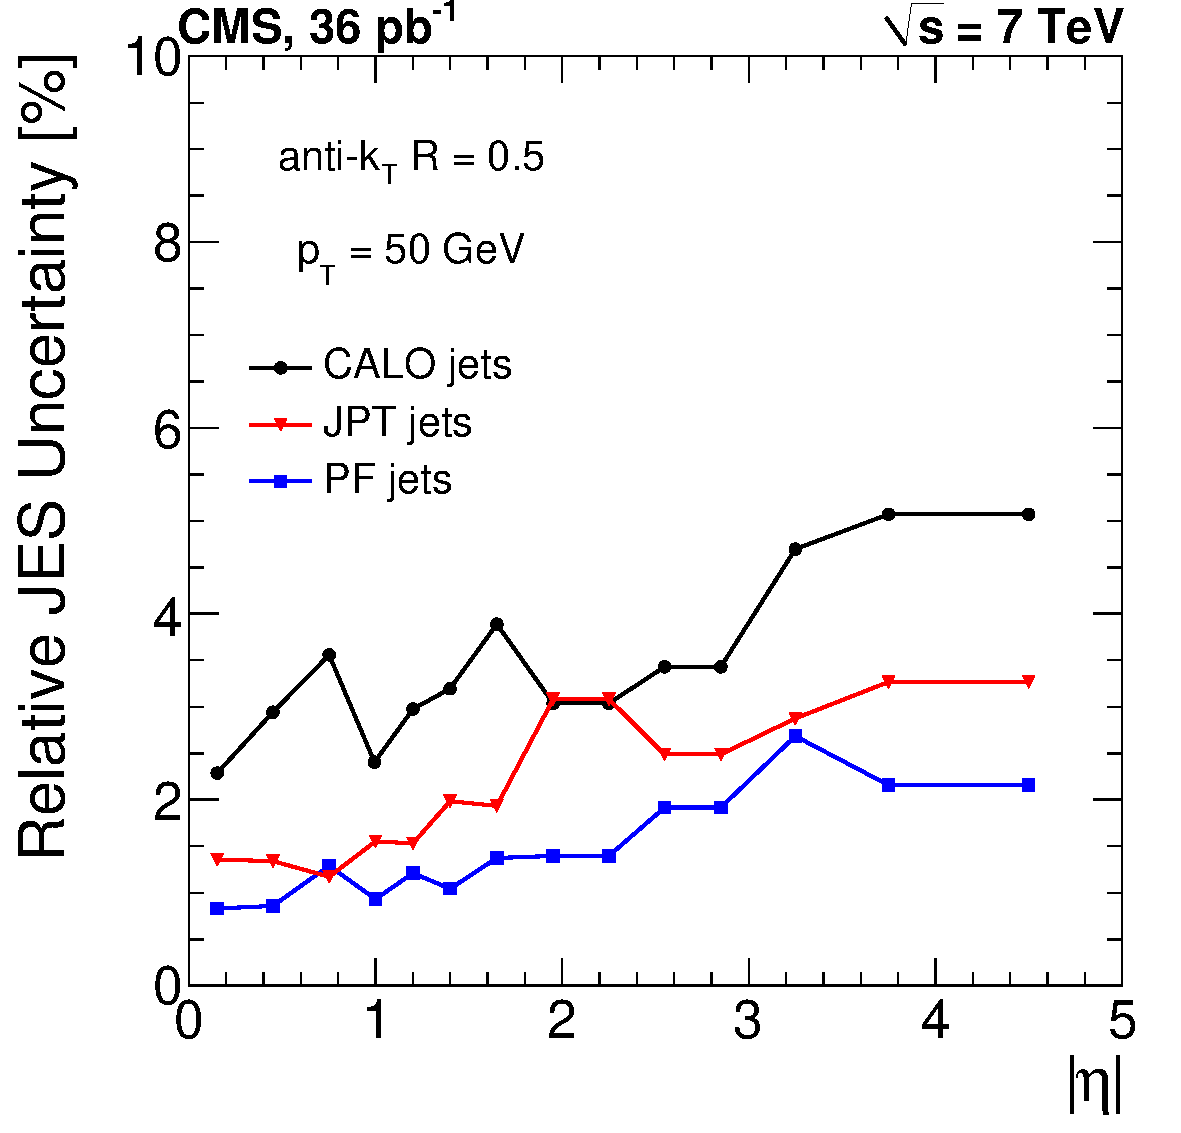
\includegraphics[width=0.45\textwidth]{Figures/JEC/ResidualUncertainty_Pt50}
    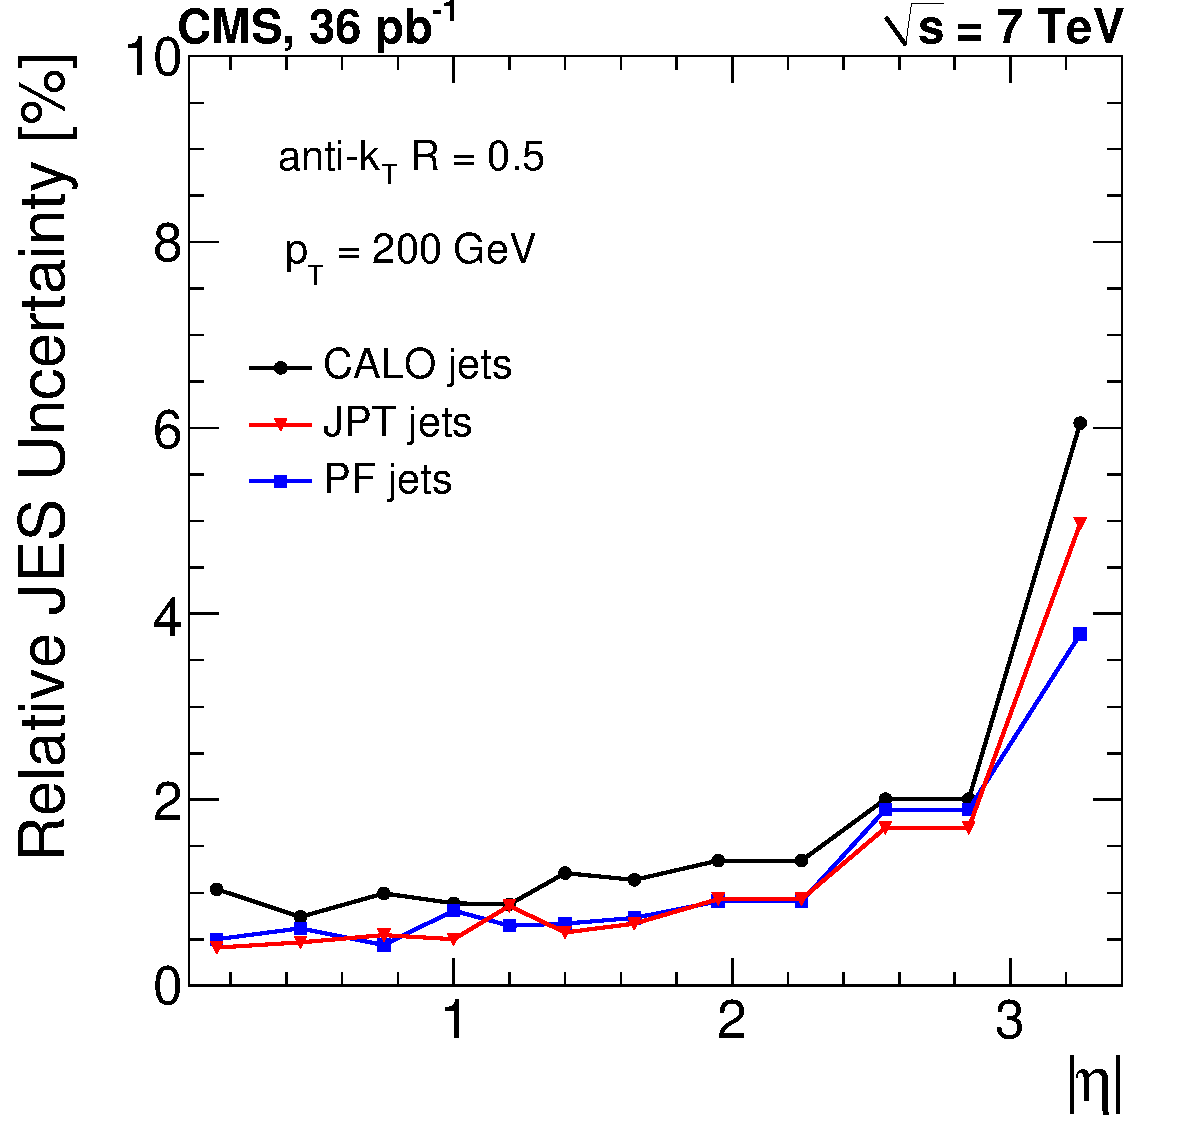
\includegraphics[width=0.45\textwidth]{Figures/JEC/ResidualUncertainty_Pt200}
    \caption{Relative jet energy residual correction uncertainty, as a function of $\eta$ for jet $\pt=50\GeV$ (left) and $\pt=200\GeV$ (right).}
    \label{fig:residual_unc}
  \end{center}
\end{figure}

\clearpage
